% !TEX encoding = MacOSRoman

\documentclass[a4paper,12pt]{article}

\usepackage{listings}
\usepackage[parfill]{parskip}
\usepackage{float}
\usepackage{graphicx}
\usepackage[swedish]{babel}
\usepackage[applemac]{inputenc}
\usepackage[margin=35mm]{geometry}
\usepackage{fancyhdr}
\usepackage[encapsulated]{CJK}
\usepackage{inconsolata}
\usepackage{amssymb,amsmath}
\usepackage{caption}
\usepackage{subcaption}


\newenvironment{ppl}{\fontfamily{ppl}\selectfont}{}
\newenvironment{inconsolata}{\texttt}{}


\DeclareGraphicsRule{.tif}{png}{.png}{`convert #1 `dirname #1`/`basename #1 .tif`.png}
\addto\captionsswedish{%
  \renewcommand{\figurename}{Figure}%
  \renewcommand{\tablename}{Table}%
  \renewcommand{\contentsname}{Table of contents}%
}

\begin{document}


\section*{Electrical and optical properties in 3C-SiC after particle irradiation}
\subsection*{Introduction}
Several studies have been done on defects created in 3C SiC when irradiated with electrons, protons, neutrons and heavier particles. Irradiation by these particles can create many types of defects, for example vacancies, interstitials and antisites. These defects manifest themselves in several ways. Some defects may act like artificial shallow donors or acceptors by creating new energy levels near the band edge, or as deeper levels in the band gap. These new energy states do of course change the electrical properties of the material in various ways. Some defects are optically radiative, and can be seen in for example PL-measurements. 

Annealing of irradiated samples can further change the properties. Simpler defects like vacancies at Si (V$_{Si}$) or C (V$_C$) sites will start to diffuse in the sample at high temperatures and may at some point encounter an interstitial (I) and recombine. Smaller defects are generally less stable than larger defect complexes, when annealed at high temperatures. The complexes are combinations of several small defects and may survive even after annealing. 

 \newpage
\pagenumbering{arabic}

\subsection*{Electrical properties}

Itoh et. al. \cite{Itoh1997} has examined proton and electron irradiated 3C using electron spin resonance (ESR) and positron annihilation spectroscopy (PAS), as well and PL and Hall measurements to find the electronic energy structure of some of the most simple defects. Figure \ref{fig:band1} shows the result of these measurements, and shows the band structure of 3C after irradiation. 

\begin{figure}[H]
\begin{center}
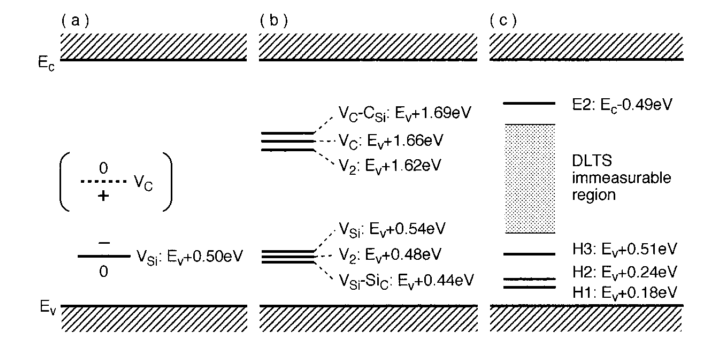
\includegraphics[scale=0.5]{band1.png}
\caption{Band diagram with some defects. Figure from \cite{Itoh1997}.
\label{fig:band1}}
\end{center}
\end{figure}

The bands in a and c are aquired by different measurement techniques. The levels in b are found by simulation. We note from a that the Si vacancy acts as an acceptor level. This level in n-doped SiC will act as an electron trap, reducing the mobility and free carrier concentration of the material. 

\begin{figure}[H]
\begin{center}
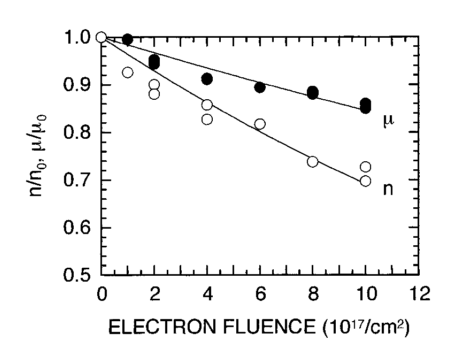
\includegraphics[scale=0.7]{mobility.png}
\caption{Hall mobility and carrier density in 3C. Figure from \cite{Itoh1997}.
\label{fig:mobility}}
\end{center}
\end{figure}

Figure \ref{fig:mobility} shows the mobility of 3C-SiC irradiated with varying electron dose. Itoh et. al. \cite{Itoh1997} explains this decrease in mobility as electron trapping in the V$_{Si}$ defect. Figure \ref{fig:resistivity1} shows a similar trend in n-doped 4H, as described by Lebedev et. al \cite{Lebedev2000}. There seems to have been no studies on resistivity change in p-doped 3C before and after particle irradiation. As described later, the vacancy defects can be more or less removed by annealing, which again restores the resistivity to the same value as before irradiation. 

\begin{figure}[H]
\begin{center}
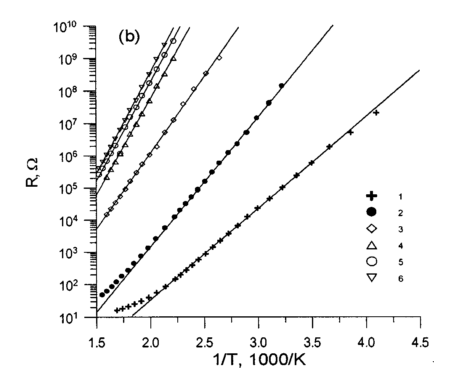
\includegraphics[scale=0.7]{resistivity1.png}
\caption{Resistivity of 4H n-doped SiC for various neutron radiation doses. Figure from \cite{Lebedev2000}.
\label{fig:resistivity1}}
\end{center}
\end{figure}

\subsection*{Optical properties}
Some of the created defects are optically radiative. Figure \ref{fig:pl1} shows some new PL-lines in 3C spectrum which do not appear before irradiation. Similar lines appear by neutron \cite{SchneiderJ.andMaierK.1993} and He-ion \cite{L.Patrick1971} irradiation. The same phenomenon should be present for proton irradiated samples too. The peak labeled E in the figure is the Si vacancy, V$_{Si}$, while the peak labeled D is a defect complex. It can be noted that before annealing the V$_{Si}$ is the highest peak, which indicates that this defect is the most common after irradiation. 

\begin{figure}[H]
\begin{center}
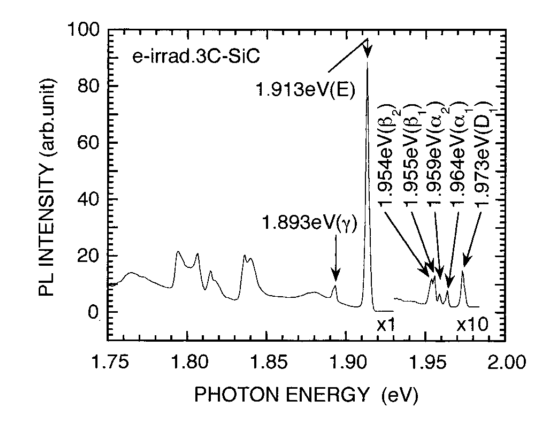
\includegraphics[scale=0.7]{pl1.png}
\caption{Some PL-lines created by electron irradiation. The spectrum is taken at 1.3 K. Figure from \cite{Itoh1997}.
\label{fig:pl1}}
\end{center}
\end{figure}

The D line is interesting due to the fact that it is a defect complex. It, as shown below, does not anneal at the same temperatures as the simpler defects. Patrick et. al. report on this D-peak for ion-irradiated samples \cite{L.Patrick1971}. They show that the ratio between the ZPL D-peak and its phonon replicas change at certain temperatures, and that there are small shifts in peak energy at these same temperatures. This is attributed to Jahn-Teller shifts at these temperatures. There are three such configurations, which are seen at $T<1.3$ K, $1.3 < T < 13$ K and $T>13$ K.  

Figure \ref{fig:D1} shows PL spectra from different polytypes. The luminescence is from the same D1 complex, showing that the complex gives strong luminescence in all four polytypes, and that the photon energy is different in different polytypes. The spectrum is for material irradiated with neutrons and subsequently annealed at 1200 C. In \cite{Kalinina2007}, the D1 defect is identified as a divacancy. 

\begin{figure}[H]
\begin{center}
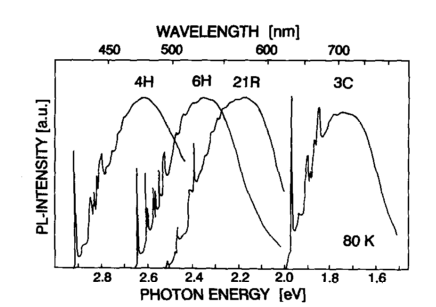
\includegraphics[scale=0.7]{D1.png}
\caption{The D1 center shown by PL in some polytypes. Figure from \cite{SchneiderJ.andMaierK.1993}.
\label{fig:D1}}
\end{center}
\end{figure}

Comparing the spectra in figures \ref{fig:pl1} and \ref{fig:D1} we see that the same defect D1 is present after both electron and neutron irradiation. The latter figure shows luminescence measurements at higher temperature than the former, which explains the merging of the phonon replicas into a band. 

\subsection*{Effects of annealing}
Annealing at different temperatures will change the defect composition of the irradiated material. This is due to defect diffusion at higher temperatures \cite{Itoh1997}. Some of the simpler defects, such as vacancies, anneal away completely. The V$_{Si}$ is annealed away at approximately 750 C \cite{Itoh1997}, whereas the V$_C$  is annealed at significantly lower temperatures \cite{Kalinina2007}. Figure \ref{fig:annealing2} shows how the Si vacancy is annealed away at certain temperatures. Itoh et. al. shows that the annealing temperature for removal of Si vacancies is the same for both electron and proton irradiated samples. 

\begin{figure}[H]
\begin{center}
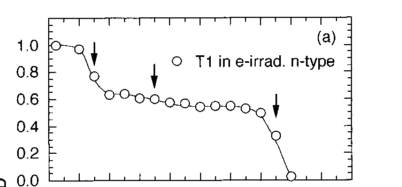
\includegraphics[scale=0.7]{annealing2.png}
\caption{Fraction of T1 (V$_{Si}$) defects remaining in n-type 3C at annealing temperatures ranging from 0 to 1000 C. Figure from \cite{Itoh1997}.
\label{fig:annealing2}}
\end{center}
\end{figure}

Some defects will however increase in number when annealing at certain temperatures. The D1 defect complex, described above, will increase in PL strength up to temperatures above 1300 C \cite{L.Patrick1971}. Bratus et. al. have shown with PL-measurements how two types of defects created by neutron irradiation will increase in number with annealing up to 1100 C \cite{Bratus2013}. This is shown in figure \ref{fig:annealing1}.

\begin{figure}[H]
\begin{center}
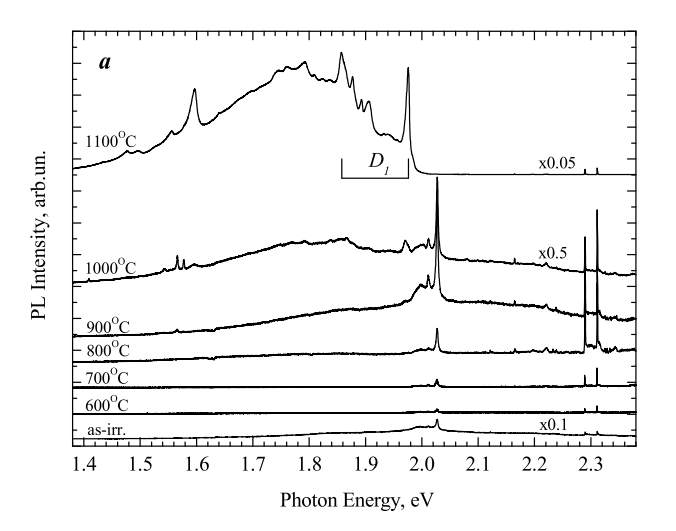
\includegraphics[scale=0.6]{annealing1.png}
\caption{PL-spectra of neutron irradiated 3C, annealed at different temperatures. The PL-measurements are done at 80 K.  Figure from \cite{Bratus2013}.
\label{fig:annealing1}}
\end{center}
\end{figure}

The peaks labeled D1 are the ZPL and its phonon replicas. These appear at 900 C annealing, and are prominent at 1100 C. Another peak appears at 1100 C, placed at approximately E = 1.6 eV. The peaks around 2.3 are thought to be Raman lines. The lines around 2.0 are described by Bratus et. al. as ''... [the] defect related to the 2.027 eV band may be a precursor of a defect associated with the D1 band''.


\newpage

\small
\bibliographystyle{unsrt}
\bibliography{../../Thesis/BibTeX/Proton_irradiation}







\end{document}








































